\documentclass[a4paper,12pt]{article} 

%%% Работа с русским языком
\usepackage{cmap}					% поиск в PDF
\usepackage{mathtext} 				% русские буквы в фомулах
\usepackage[T2A]{fontenc}			% кодировка
\usepackage[utf8]{inputenc}			% кодировка исходного текста
\usepackage[english,russian]{babel}	% локализация и переносы

%%% Дополнительная работа с математикой
\usepackage{amsmath,amsfonts,amssymb,amsthm,mathtools, gensymb} % AMS
\usepackage{icomma} % "Умная" запятая: $0,2$    ф--- число, $0, 2$ --- перечисление

%%Таблица
\usepackage[table,xcdraw]{xcolor}
\usepackage{caption}
\usepackage{floatrow}
\floatsetup[table]{capposition=top}
\floatsetup[wrapfigure]{capposition=bottom}
\usepackage{multirow}

\usepackage{hyperref}

%Отступы и поля 
\textwidth=18cm
\oddsidemargin=-1cm
\topmargin=-2cm
\textheight=25cm


%% Номера формул
\mathtoolsset{showonlyrefs=false} % Показывать номера только у тех формул, на которые есть \ref{} в тексте.

%% Шрифты
\usepackage{euscript}	 % Шрифт Евклид
\usepackage{mathrsfs} % Красивый матшрифт

%% Свои команды
\DeclareMathOperator{\sgn}{\mathop{sgn}}

%% Перенос знаков в формулах (по Львовскому)
\newcommand*{\hm}[1]{#1\nobreak\discretionary{}
{\hbox{$\mathsurround=0pt #1$}}{}}

%% Стиль страницы
\usepackage{fancyhdr}

%% Для рисунков
\usepackage{graphicx}
\usepackage[export]{adjustbox}
\usepackage{float}
\usepackage{ragged2e}
\usepackage{wrapfig}

\pagestyle{fancy}
\begin{document}
\begin{titlepage}
\begin{center}
%\vspace*{1cm}
\large{\small ФЕДЕРАЛЬНОЕ ГОСУДАРСТВЕННОЕ АВТОНОМНОЕ ОБРАЗОВАТЕЛЬНОЕ\\ УЧРЕЖДЕНИЕ ВЫСШЕГО ОБРАЗОВАНИЯ \\ МОСКОВСКИЙ ФИЗИКО-ТЕХНИЧЕСКИЙ ИНСТИТУТ\\ (НАЦИОНАЛЬНЫЙ ИССЛЕДОВАТЕЛЬСКИЙ УНИВЕРСИТЕТ)\\ ФАКУЛЬТЕТ АЭРОКОСМИЧЕСКИХ ТЕХНОЛОГИЙ}
\vfill
\line(1,0){490}\\[1mm]
\huge{Лабораторная работа 10.1}\\
\huge\textbf{Электронный парамагнитный резонанс}\\
\line(1,0){490}\\[1mm]
\vfill
\begin{flushright}
\normalsize{Рогозин Владимир}\\
\normalsize{\textbf{Группа Б03-106}}\\
\end{flushright}
\end{center}
\end{titlepage}
\fancyhead[L] {Работа 10.1}

\textbf{Цель работы}:
пронаблюдать и изучить эффект парамагнитного резонанса в дифенилпикрилгидразиле, сокращённо обозначаемом ДФПГ. Определить эффективный $g$-фактор вещества, а также ширину линии ЭПР.


% \textbf{Оборудование}:
% лазер; кассета с набором сеток разного
% периода; линзы; щель с микрометрическим винтом; оптический стол
% c набором рейтеров и крепёжных винтов; экран; линейка.


\section{Теоретические сведения}

\subsection{Постановка эксперимента по электронному парамагнитному резонансу}
В методе ЭПР изучается резонансное поглощение переменного электромагнитного поля в
образце в зависимости от контролируемых экспериментатором внешних условий:
постоянного магнитного поля, частоты колебаний переменного поля, температуры.
\begin{figure}[H]\label{fig: Zeeman effect}
    \centering
    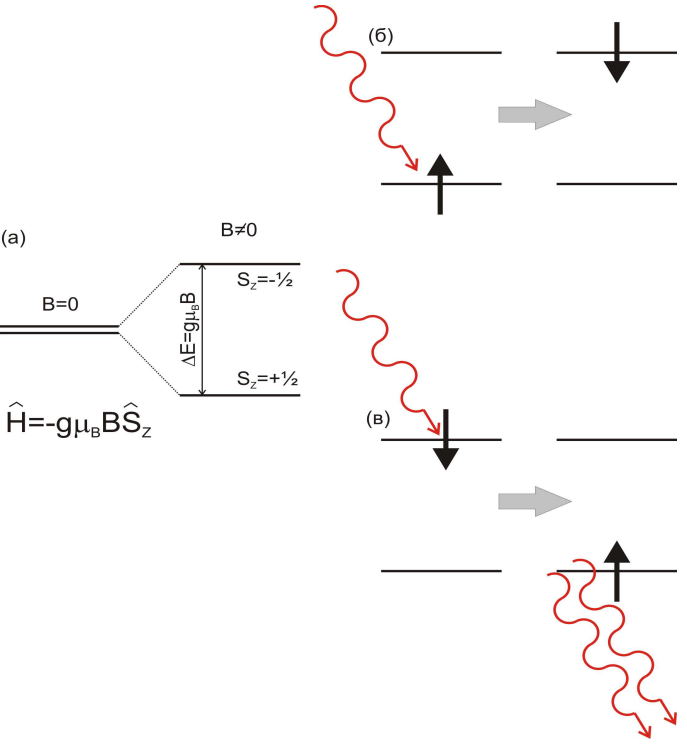
\includegraphics[width = 0.78\textwidth]{Zeeman effect.png}
    \caption{(a) Зеемановское расщепление спинового уровня в магнитном поле. (б) Переход
        между подуровнями «снизу-вверх» с поглощением фотона резонансной частоты $h\nu = g \mu_B B$. (в) Переход между подуровнями «сверху-вниз» с излучением дополнительного фотона резонансной частоты.}
\end{figure}


Простейшей моделью для рассмотрения ЭПР является система из невзаимодействующих
частиц со спином $S= 1 / 2$ , помещённая во внешнее магнитное поле. В отсутствие
магнитного поля энергии состояний с проекцией спина $S_z = \pm 1 / 2$ совпадают. Из-за \textit{эффекта Зеемана} в магнитном поле энергии состояний с различными проекциями спина начинают различаться. Если направить на нашу систему поток излучения (поток фотонов) с энергией, равной разнице энергий этих состояний $h\nu = g \mu_B B$ , то станут возможны индуцированные переходы между состояниями. Эти переходы происходят с поглощением (рис. \hyperref[fig: Zeeman effect]{1-б}) или испусканием (рис. \hyperref[fig: Zeeman effect]{1-в}) фотона в зависимости от того, в каком из состояний была система до взаимодействия с излучением. За исключением очень низких температур, заселённость обоих спиновых подуровней с $S_z = \pm 1 / 2$ близка. В состоянии теплового равновесия нижний энергетический уровень более заселён, поэтому наблюдается поглощение электромагнитного излучения. 

Для наблюдения этого поглощения необходимо резонансное совпадение частоты излучения с
зеемановским расщеплением спиновых подуровней. Измеряемой в эксперименте величиной является поглощаемая в образце мощность излучения. В колебательном контуре, и в микроволновом резонаторе области колебаний электрического и магнитного поля оказываются пространственно разделены: в колебательном контуре электрическое поле колеблется в конденсаторе, а магнитное -- в катушке индуктивности, в микроволновом резонаторе в пучности магнитного поля электрическое поле обращается в ноль. Это позволяет поместить образец в такое место установки, в котором есть только переменное магнитное поле, причём поляризация этого поля тоже известна. 

Поглощение переменного магнитного поля в образце описывается мнимой частью магнитной
восприимчивости \fbox{$P_\text{погл.} = \frac{1}{2}\omega b^2\chi''(\omega , B)$} , где $\omega$ -- частота переменного поля, $b$ -- амплитуда однородного по малому образцу переменного поля и $B$ -- постоянное магнитное поле, а $\chi''$ -- мнимая часть высокочастотной магнитной восприимчивости. В данной работе исследуется парамагнетик при комнатной температуре, восприимчивость и намагниченность которого в условиях эксперимента малы. Поэтому далее не учитывается различие между индукцией и напряжённостью магнитного поля и считается поле в образце совпадающим с полем в воздушном зазоре электромагнита.

Таким образом, в ходе ЭПР-эксперимента изучается зависимость мнимой части высокочастотной восприимчивости от магнитного поля. При некоторых условиях (подбор
которых и составляет техническую сторону ЭПР-эксперимента) может возникать резонансное увеличение мнимой части высокочастотной восприимчивости.

\subsection{Физические причины возникновения резонансного поглощения в парамагнетике}
Простейшей системой для изучения методом ЭПР является парамагнетик -- система слабо
взаимодействующих атомов, ионов или молекул, обладающих собственным магнитным
моментом. Пренебрегая взаимодействием, можно рассмотреть поведение магнитного диполя в постоянном и переменном магнитном поле. 

В «классическом» подходе рассматривается прецессия магнитного момента во внешнем поле при отклонении магнитного момента от равновесия. При отклонении диполя от равновесия возникает возвращающий механический момент $T = M \times B$. Так как магнитный и механический момент иона связаны друг с другом \textit{гиромагнитным отношением} $\gamma$ как $M = \gamma I$ , где -- это полный момент импульса, то с учётом уравнения динамики
$\frac{dI}{dt} = T$ получим уравнение прецессии магнитного момента \fbox{$\frac{dM}{dt} =\gamma M \times B$}. При отклонении магнитного момента от направления магнитного поля возникает незатухающая прецессия вокруг направления поля с угловой скоростью $\Omega = -\gamma B$, частота этой прецесси называется \textit{ларморовской}. При совпадении частоты переменного поля с ларморовской частотой возможно возникновение резонансного поглощения.

При квантовомеханическом способе описания рассматривается структура расщеплённых в
магнитном поле термов атомов (ионов или молекул) и переходы между расщеплёнными подуровнями (рис. \hyperref[fig: Zeeman effect]{1}). Расщепление терма свободного иона (или молекулы) определяется \textit{спектроскопическим фактором Ланде} ($g$-фактором Ланде): $E(m_J)=g \mu_B B m_J$. В кристалле ионы или молекулы не свободны, на них действует электрическое поле соседей, под действием которого фиксируется пространственное расположение электронных облаков внешних оболочек. В таких случаях расщепление уровня иона описывают эффективным g-фактором \fbox{$E(m_J)=g_\text{эфф.} \mu_B B m_J$}, в реальных кристаллах эффективный $g$-фактор может быть анизотропен. Простым оказывается случай, когда орбитального вклада в магнитный момент неспаренных электронов нет. В этом случае полный момент связан только со спином и расщепление терма в магнитном поле происходит по проекции спина. Именно этот случай и реализуется в данной работе. В таком слуачае эффективный $g$-фактор такого соединения оказывается очень близок к чистоспиновому значению 2.0.

При совпадении энергии фотона с расстоянием между спиновыми подуровнями возможны резонансные переходы с поглощением или излучением фотона. По правилам отбора при поглощении или излучении фотона наиболее вероятны переходы с изменением проекции спина на единицу Частота такого фотона $h\nu = g_\text{эфф.} \mu_B B$ . Как и при рассмотрении прецессии получили, что характерная частота поглощения или испускания фотонов линейна по постоянному магнитному полю. Как и при рассмотрении прецессии получили, что характерная частота поглощения или испускания фотонов линейна по постоянному магнитному полю. Независимое измерение резонансного поля и частоты высокочастотного электромагнитного поля позволяет определить эффективный $g$-фактор: \fbox{$g_\text{эфф.} = {h\nu}/{\mu_B B}$}.

\subsection{Процессы релаксации и ширина линии ЭПР}
В отсутствие взаимодействия атомов или молекул парамагнетика между собой и с термостатом, спиновые подуровни имели бы нулевую ширину. Тогда после поглощения
кванта энергии электромагнитного поля спин оставался бы в высокоэнергетичном состоянии
бесконечное время. Эта картина, очевидно, не учитывает спонтанные переходы между подуровнями. Спонтанные переходы связаны с тем, что в реальных системах всегда есть процессы релаксации, которые стремятся поддерживать термодинамически равновесную заселённость спиновых подуровней. Эти процессы обеспечивают конечное время жизни в возбуждённом состоянии, что означает размытие этого уровня до полосы некоторой конечной ширины (рис. \hyperref[fig: Level splitting]{2}). 
\begin{figure}\label{fig: Level splitting}
    \centering
    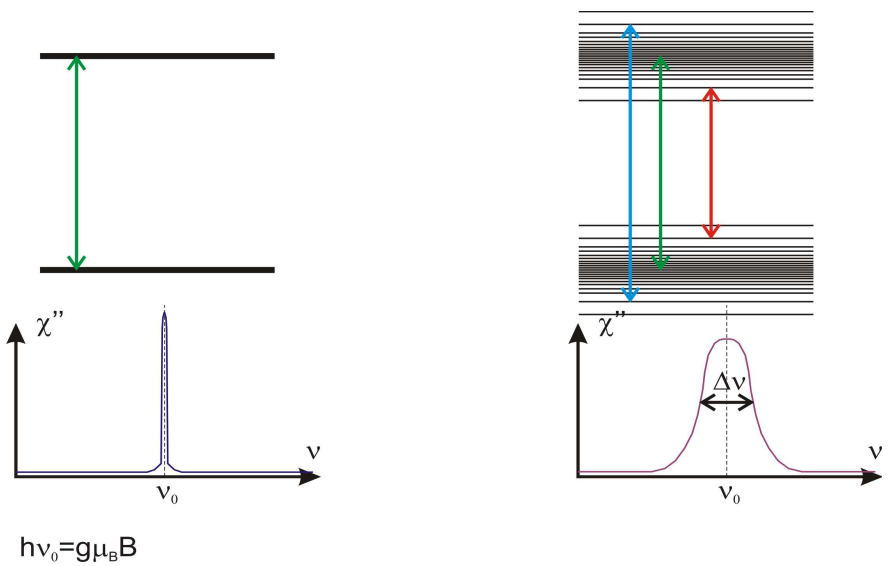
\includegraphics[width = 0.9\textwidth]{Level splitting.png}
    \caption{Размытие спиновых подуровней из-за процессов спин-спиновой релаксации,
            возможные резонансные переходы и форма линии поглощения.}
\end{figure}

Резонансное поглощение тогда возможно в некотором интервале частот вблизи резонансной и наблюдаемая линия магнитного резонанса приобретает конечную ширину. Этот вывод не зависит от подробностей того, как именно устроены процессы релаксации. Из ширины линии ЭПР можно извлечь некоторую информацию об этих процессах, что является одним из применений метода ЭПР. 

Выделяют два вида процессов релаксации: \textit{спин-решёточную} релаксацию, когда энергия возбуждённого спинового состояния отдаётся в колебания решётки, и \textit{спин-решёточную} релаксацию, связанную с взаимодействием спинов друг с другом. Такое разделение связано с тем, что во множестве случаев характерные времена установления теплового равновесия в подсистеме взаимодействующих магнитных моментов оказываются много меньше, чем время окончательной термализации этих магнитных моментов с решёткой кристалла, в котором они находятся. Эти два вида процессов релаксации можно различить по их температурной зависимости: при температурах порядка дебаевской и выше вероятность спин-фононного процесса увеличивается с температурой, а вероятность спин-спиновой релаксации обычно остаётся постоянной.

Кроме процессов релаксации внутри образца в наблюдаемую ширину линии ЭПР даёт вклад
и неоднородность магнитного поля на размере образца. В простых ЭПР спектрометрах,
используемых в данной работе, вклад неоднородности магнитного поля может быть
заметным.

\section{Экспериментальная установка}
В работе исследуется ЭПР в дифенилпикрилгидразиле, сокращённо обозначаемом ДФПГ.

Схема установки показана на рисунке \hyperref[fig: Exp setup]{4}. Переменное электромагнитное поле на частоте $\sim100$ МГц создаётся высокочастотным генератором, постоянное магнитное поле создаётся электромагнитом.
\begin{figure}\label{fig: Exp setup}
    \centering
    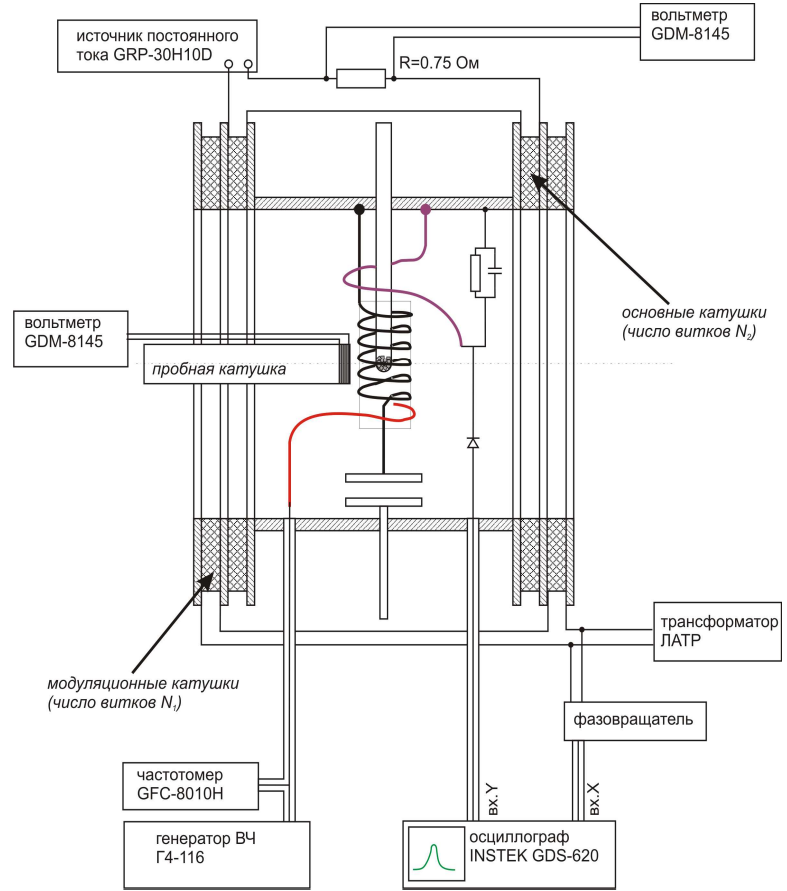
\includegraphics[width = \textwidth]{Exp setup.png}
    \caption{Схема установки}
\end{figure}

Поглощаемая мощность $P_\text{погл.} = \frac{1}{2}\omega b^2\chi''(\omega , B)$ пропорциональна квадрату амплитуды переменного поля $b$. Для увеличения чувствительности эксперимента образец помещают в катушку индуктивности колебательного контура. Колебательный контур состоит из катушки индуктивности и плоского конденсатора. Генератор высокой частоты не соединён с контуром непосредственно: для возбуждения колебаний в контуре служит электродинамическая связь в виде антенны, соединённой с выходом генератора. Излучаемое антенной электромагнитное поле возбуждает колебания в контуре. Для определения амплитуды этих вынужденных колебаний рядом с катушкой индуктивности контура расположен виток приёмной катушки детектора. Колебания магнитного поля в катушке индуктивности наводят ЭДС индукции в этом витке. Частота колебаний этой ЭДС индукции соответствует $\sim100$ МГц, для измерения этого сигнала он подаётся на детектор. Детектором является высокочастотный диод, при малых амплитудах напряжения детектирование происходит за счёт нелинейности его вольт амперной характеристики и среднее напряжение на диоде оказывается пропорционально квадрату амплитуды переменного напряжения, то есть квадрату амплитуды переменного магнитного поля в катушке индуктивности. В цепь детектора подключён осциллограф. Для создания магнитного поля используется электромагнит, состоящий из пары разнесённых катушек. Ток через электромагнит контролируется по падению напряжения на резисторе, включённом в цепь питания катушек. Дополнительно к основным катушкам имеется пара модуляционных катушек, в которые могут создавать переменное поле малой амплитуды. Для создания переменного поля к катушкам прикладывается напряжение с трансформатора ЛАТР, частота колебаний переменного поля соответствует частоте колебаний напряжения в сети переменного тока. Калибровка электромагнита осуществляется по измерению наводимой ЭДС индукции в пробной катушке известной геометрии при подаче переменного тока в соответствующие катушки электромагнита.

Для выполнения измерений генератор высокой частоты настраивается на резонансную частоту колебательного контура. Амплитуда колебаний поля в катушке контура определяется добротностью контура и уменьшится при возникновении поглощения в образце. Поэтому
необходимо подстроить ток через катушки электромагнита до возникновения этого поглощения. Дополнительная модуляция поля используется для облегчения этой настройки.

\section{Обработка данных}

\subsection{Определение добротности и резонансной частоты контура}
\begin{enumerate}
    \item
    Включим генератор, установим частоту, близкую к резонансной частоте колебательного контура $f_\text{рез.} \approx 163$ Мгц, выставим частоту $\Omega = 1000$ Гц и глубину $m = 10 \%$ амплитудной модуляции, сигнал подадим на осциллограф.
    \item
    Найдём точное значение резонансной частоты $f_\text{рез.} = 160,6181$ МГц. После этого измерим $f_{0,5}$ и $f_{-0,5}$ -- частоты, на которых достигается половина амплитуды сигнала при расстройке генератора в сторону больших и маленьких частот.
    \begin{table}[H]
        \centering
        \begin{tabular}{|
            >{\columncolor[HTML]{FFFFFF}}c |
            >{\columncolor[HTML]{FFFFFF}}c |
            >{\columncolor[HTML]{FFFFFF}}c |
            >{\columncolor[HTML]{FFFFFF}}c |}
            \hline
            {\color[HTML]{000000} $f_\text{рез.}$, МГц} & {\color[HTML]{000000} $f_{0,5}$, МГц} & {\color[HTML]{000000} $f_{-0,5}$, МГц} & {\color[HTML]{000000} $Q_0$, отн. ед.} \\ \hline
            {\color[HTML]{000000} $160,61 \pm 0,05$}            & {\color[HTML]{000000} $160,91 \pm 0,05$}      & {\color[HTML]{000000} $160,26 \pm 0,05$}       & {\color[HTML]{000000} $247 \pm 19$}           \\ \hline
        \end{tabular}
        \caption{Резонансная частота и добротность контура}
    \end{table}
    
\end{enumerate}

\subsection{Калибровка поля электромагнита и определение g-фактора}
\begin{enumerate}
    \item
    Подключим основные катушки к источнику постоянного тока, а модуляционные катушки к
    трансформатору ЛАТР. Подадим на модуляционные катушки напряжение $\sim 40$ В. Плавно увеличивая постоянное напряжение, подаваемое на основные катушки, добьёмся
    возникновения на экране осциллографа картины резонансного поглощения. 
    \item
    Найдём связь между падением напряжения на резисторе в цепи основной катушки и магнитным полем. Для этого переключим основные катушки на ЛАТР и установим ток через катушки близкий к значению тока при наблюдении резонансного поглощения. Внесём пробную катушку в центр магнита, и зная её параметры и напряжение, сможем найти магнитное поле внутри катушки по формуле \fbox{$B = \frac{V}{nS\omega}.$}   
    \begin{table}[H]\label{tab: coil params}
        \centering
        \begin{tabular}{|
            >{\columncolor[HTML]{FFFFFF}}c |
            >{\columncolor[HTML]{FFFFFF}}c |
            >{\columncolor[HTML]{FFFFFF}}c |}
            \hline
            {\color[HTML]{000000} $n$, витков} & {\color[HTML]{000000} $d$, мм}   & {\color[HTML]{000000} $V$, мВ}   \\ \hline
            {\color[HTML]{000000} $45$} & {\color[HTML]{000000} $15,2 \pm 0,1$} & {\color[HTML]{000000} $16,6 \pm 0,2$} \\ \hline
        \end{tabular}
        \caption{Параметры пробной катушки и напряжение в цепи}
    \end{table}
    \[B = (6,47 \pm 0,12)\text{ мТл,} \quad \varepsilon_B \approx 1,8\%.\]
    \item 
    Теперь, используя формулу \fbox{$g = \frac{h\nu}{\mu_B B}$}, $\mu_B = 927,4 \cdot 10^{-26} \text{ Дж/Тл}$ -- магнетон Бора, вычислим эффективный $g$-фактор:
    \[g_\text{эфф.} = 1,77 \pm 0,03 \quad \varepsilon_g \approx 1,8\%.\]
\end{enumerate} 

\subsection{Определение ширины линии ЭПР}
\begin{enumerate}
    \item
    Подадим на $X$-канал осциллографа напряжение, прикладываемое к модуляционным катушкам и будем наблюдать сигнал в $XY$-режиме. Подберём напряжение на модуляционных катушках так, чтобы на экране осциллографа наблюдать зависимость поглощения в образце от приложенного переменного поля.
    \item 
    Для определения ширины линии ЭПР определим по экрану осциллографа полный размах
    модулирующего поля $A_\text{полн}$ и полную ширину кривой резонансного поглощения на полувысоте $A_{1/2}$. С помощью пробной катушки измерим определим величину поля по формуле \fbox{$B_\text{мод} = \sqrt{2} \frac{V}{nS\omega}$}. Результаты приведены ниже:
    \[B_\text{мод} = (2,34 \pm 0,03)\text{ мТл,} \quad \varepsilon_{B_\text{мод}} \approx 1,3\%.\]
    \begin{table}[H]\label{tab: resonance width}
        \centering
        \begin{tabular}{|
            >{\columncolor[HTML]{FFFFFF}}c |
            >{\columncolor[HTML]{FFFFFF}}c |
            >{\columncolor[HTML]{FFFFFF}}c |}
            \hline
            {\color[HTML]{000000} $A_\text{полн}$, дел.} & {\color[HTML]{000000} $A_{1/2}$, дел.} & {\color[HTML]{000000} $V$, мВ} \\ \hline
            {\color[HTML]{000000} $5,8 \pm 0,1$}             & {\color[HTML]{000000} $0,8 \pm 0,1$}       & {\color[HTML]{000000} $4,25$}  \\ \hline
        \end{tabular}
        \caption{Данные измерений}
    \end{table}
    Теперь рассчитаем полуширину на полувысоте линии резонансного поглощения как \\ \fbox{$\Delta B = \frac{A_{1/2}}{A_\text{полн}}B_\text{мод}$}.
    \[\Delta B = (32,28 \pm 4,04)\text{ Гс}, \quad \varepsilon_{\Delta B}  \approx 12,5\%.\]
    
\end{enumerate}    

\section{Вывод}
В данной работе исследовалось явление электронного парамагнитного резонанса. В результате:
\begin{itemize}
    \item
\end{itemize}

\newpage
%%%%%%%%%%%%%%%%%%%%%%%%% Графики

%%%%%%%%%%%%%%%%%%%%%%%%%
\end{document}
